\chapter{Metodología}

\section{Descripción de la metodología aplicada}

\begin{center}
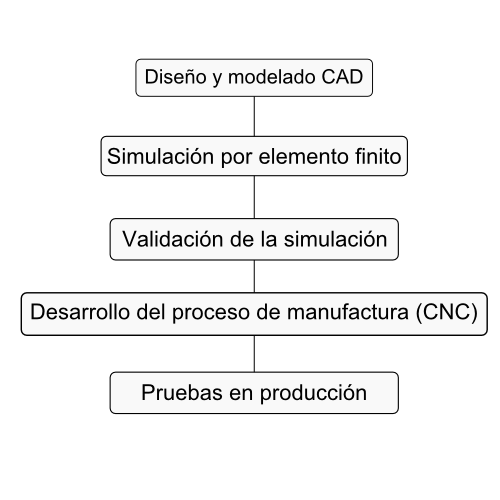
\includegraphics[scale=0.75]{src/ch3/diagrama_metodologia.png}
\captionof{figure}{Metodología del proyecto}
\label{fig:diagrama_metodologia}
\end{center}

\section{Análisis por elementos finitos}

\subsection{Consideraciones generales}

Para realizar el análisis por elementos finitos se han tomado sólo los elementos formadores que 
tienen influencia directa o contacto sobre el formado del tubo, quitando todos los elementos 
del troquel adicionales. Además, los formadores se han considerado como elementos rígidos, 
para simplificar y agilizar el análisis numérico, al permanecer sus características geométricas 
invariables, siendo solamente el blank un sólido deformable.

\subsection{Geometrías y partes}

En ANSYS/LS-DYNA el concepto de parte es fundamental e incluye dentro de este a todos aquellos 
elementos que comparten el tipo de material, tipo de elemento y sección. Así, es preferible que 
cada componente o pieza se defina como una parte, aun cuando las propiedades elasto-plásticas 
sean iguales. Por ello, para cada una de los componentes del troquel se definió un material 
distinto (aunque con las mismas propiedades).

\begin{center}
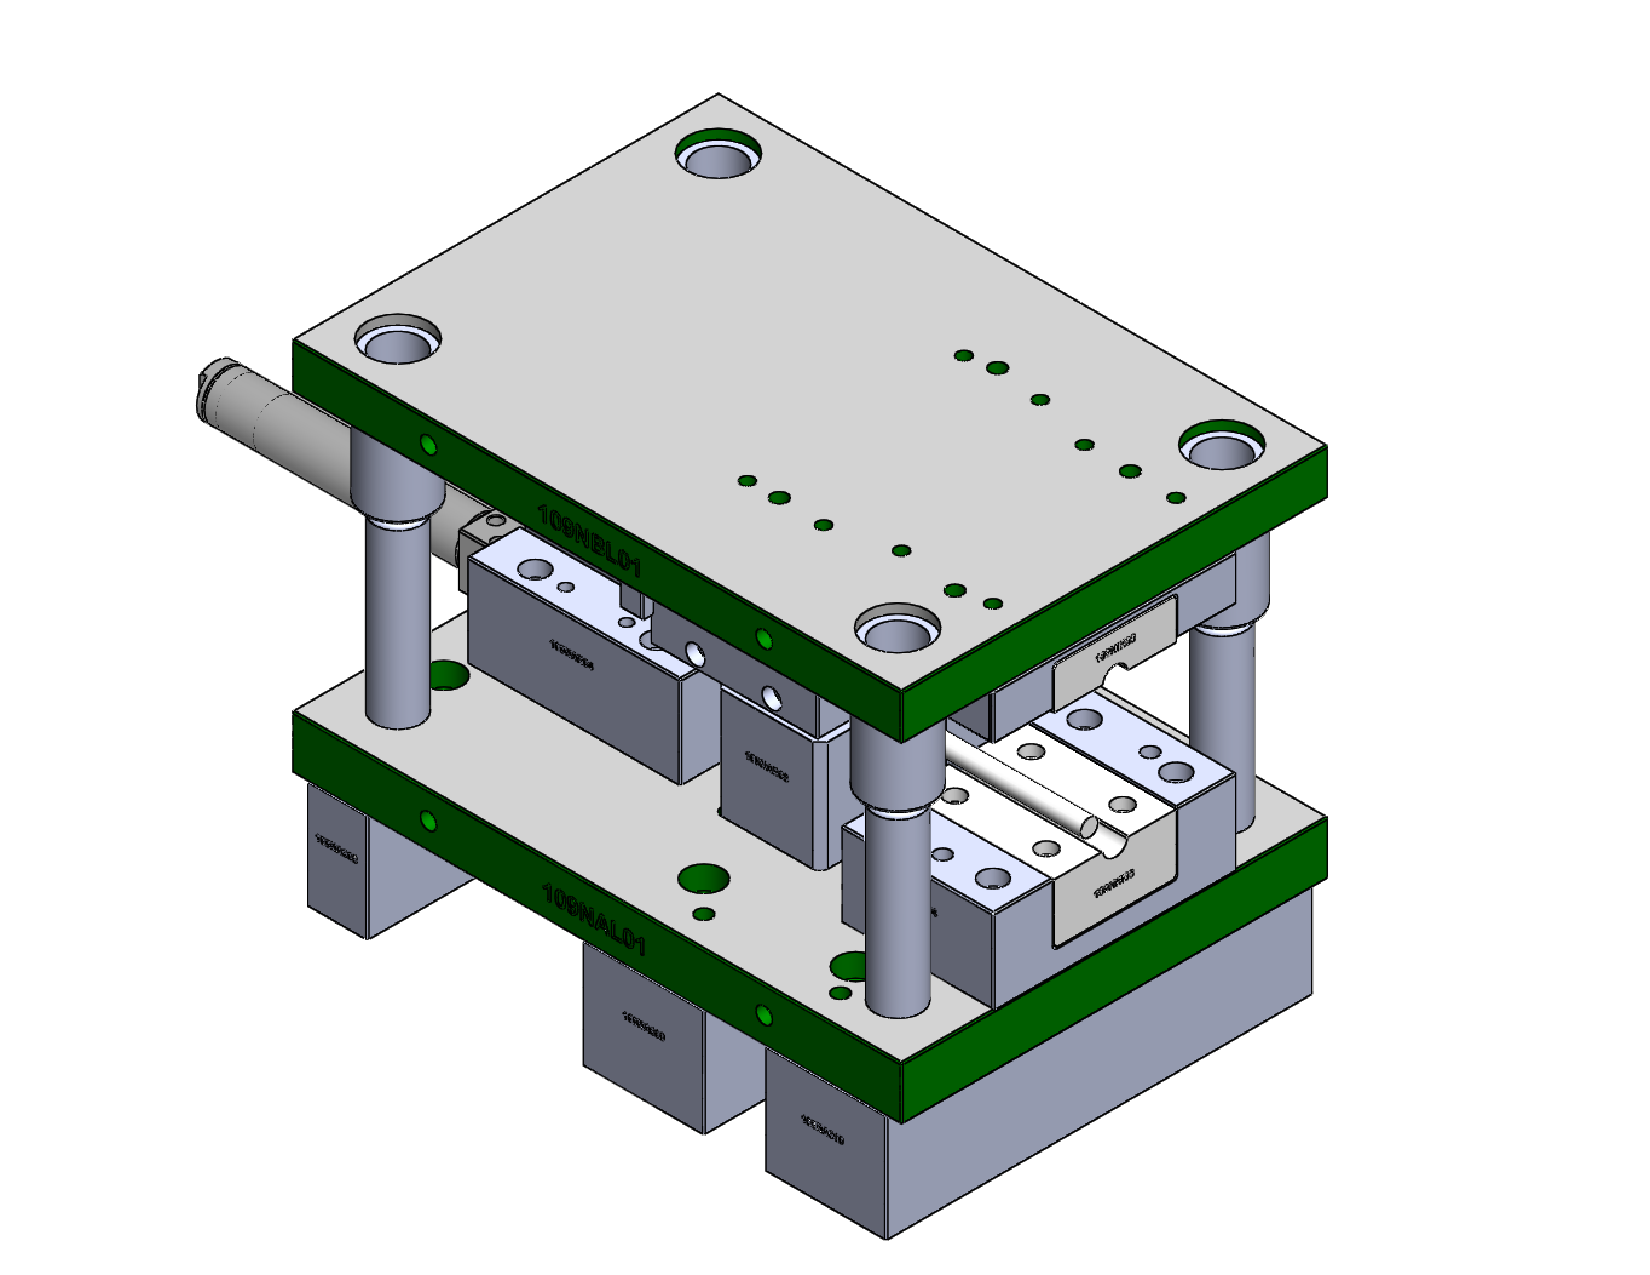
\includegraphics[scale=0.55]{src/ch3/troquel}
\captionof{figure}{Vista completa del troquel}
\label{fig:all_tool}
\end{center}

\subsection{Modelo constitutivo}

Se utilizó un modelo de tipo \textit{Piecewise Linear Plasticity}, el cual es un modelo multilineal 
que permite utilizar una curva esfuerzo-deformación y la dependencia de la tasa de deformación 
como datos de entrada para definir el comportamiento plástico del material. Para cuantificar 
la tasa de deformación este modelo utiliza la relación de Cowper-Symonds.\\

\begin{equation}
\[{{\sigma }_{y}}\left( \varepsilon _{eff}^{P},\dot{\varepsilon }_{eff}^{P} \right)={{\sigma }_{y}}\left( \varepsilon _{eff}^{P} \right)\left[ 1+{{\left( \frac{\dot{\varepsilon }_{eff}^{P}}{C} \right)}^{\frac{1}{P}}} \right]\]
\end{equation}

En los componentes del troquel se utilizó un modelo rígido, para el cual sólo es necesario 
especificar las propiedades elásticas. Los componentes rígidos, normalmente, permiten la 
aplicación de condiciones de desplazamiento utilizando el identificador (ID) de la parte, además 
se pueden asignar propiedades de inercia o velocidades iniciales. En este caso, no se 
especificaron propiedades adicionales, lo cual implica que ANSYS/LS-DYNA calcule automáticamente 
las propiedades inerciales basadas en el modelo de elemento finito.\\

Para crear los materiales de cada uno de los componentes se utilizó un pequeño \textit{script}, 
que se muestra a continuación:

\begin{apdl}
! Para el formador inferior
MP,EX,2,29E6 ! psi
MP,NUXY,2,0.3 ! 
MP,DENS,2,0.00073 ! lbf s^2 / in^4
EDMP,rigid,2,7,7

! Formador superior izquierdo
MP,EX,3,29E6 ! psi
MP,NUXY,3,0.3 ! 
MP,DENS,3,0.00073 ! lbf s^2 / in^4
EDMP,rigid,3,6,7

! Formador superior derecho
MP,EX,4,29E6 ! psi
MP,NUXY,4,0.3 ! 
MP,DENS,4,0.00073 ! lbf s^2 / in^4
EDMP,rigid,4,6,7

! Leva izquierda
MP,EX,5,29E6 ! psi
MP,NUXY,5,0.3 ! 
MP,DENS,5,0.00073 ! lbf s^2 / in^4
EDMP,rigid,5,6,4

! Leva derecha
MP,EX,6,29E6 ! psi
MP,NUXY,6,0.3 ! 
MP,DENS,6,0.00073 ! lbf s^2 / in^4
EDMP,rigid,6,6,4

! Para el blank
! Propiedades elásticas
MP,EX,1,29E6 ! psi
MP,NUXY,1,0.3 ! 
MP,DENS,1,0.00073 ! lbf s^2 / in^4

! define array for effective plastic true strain data
*dim,strn,,6
! define array for effective total true stress data
*dim,strs,,6

! strain (in/in)
strn(1)= 0.0, 0.0293, 0.0772, 0.1562, 0.2356, 0.344943

! stress (psi)
strs(1)=52489.4,60585.8,70710,76809.3,80244.3,82574.1

! curve #1: abscissa=strain & ordinate=stress
edcurve,add,1,strn,strs 

! specify power law #8 for material (MAT) #1
TB,PLAW,1,,,8  ! Piecewise Linear Plasticity

! use load curve #1 for stress/strain data
TBDATA,1,52e3 ! Yield stress (psi)
TBDATA,3,.75 ! Failure strain
TBDATA,4,40.0 ! C (strain rate parameter)
TBDATA,5,0.1 ! P (strain rate parameter)
TBDATA,6,1 ! Load Curve ID
\end{apdl}



% Tabla de propiedades

\begin{table}[h]
\centering
\caption{Propiedades del acero AISI 1018}
\label{}
\begin{tabular}{p{4cm} p{4cm}} \hline
Propiedad & Magnitud (unidades) \\
\hline
Módulo elástico & 29 000 (ksi) \\
Densidad & 0.00073 ($lbf s^2/in^4$) \\
Esfuerzo de fluencia & 52 000 (psi) \\
Coeficiente de Poisson & 0.3 \\
C & 40 ($s^{-1}$) \\
P & 5 \\
\hline
\end{tabular}
\label{tab:material_properties}
\end{table}


\subsection{Mallado}

Para el mallado de la pieza de trabajo se utilizó el elemento \texttt{SOLID164} 
( ver figura \ref{fig:solid164} ), el cual es un sólido de 8 nodos, que puede ser utilizado con el modelo 
constitutivo descrito en la sección anterior. Este elemento utiliza, por defecto, integración reducida 
(un punto de integración), el cual tiene la ventaja de reducir el tiempo de cómputo y adiciona 
robustez para el caso de grandes deformaciones. ~\cite{lsdyna-ansys-manual}

\begin{center}
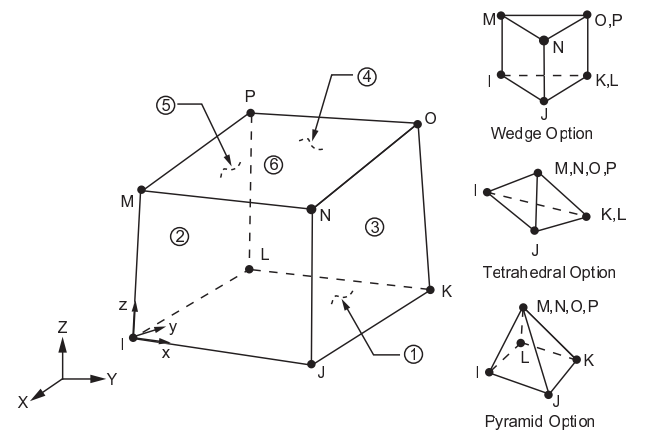
\includegraphics[scale=0.65]{src/ch3/solid164.png}
\captionof{figure}{Elemento SOLID164}
\label{fig:solid164}
\end{center}

En los componentes del troquel se mallaron solamente las áreas que están en contacto directo con el 
\textit{blank} durante el proceso de formado, con la finalidad de reducir el número de elementos del modelo. 
Se utilizaron elementos \texttt{SHELL163} para realizar el mallado. Los parámetros requeridos para 
este elemento se indican en la tabla \ref{tab:shell_param}

\begin{center}
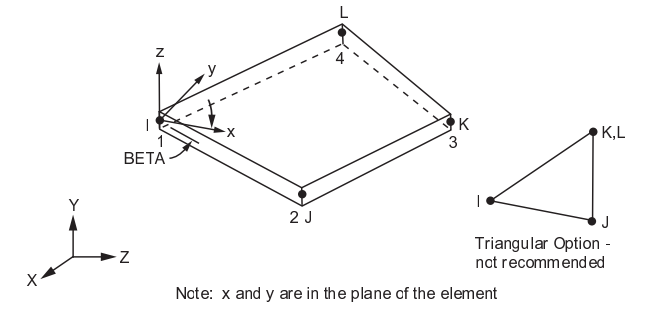
\includegraphics[scale=0.65]{src/ch3/shell163.png}
\captionof{figure}{Elemento SHELL163}
\label{fig:shell163}
\end{center}


% Tabla de propiedades para elemento SHELL163
\begin{table}[h]
\centering
\caption{Parámetros utilizados para el elemento SHELL163}
\label{}
\begin{tabular}{p{6cm} p{6cm}} \hline
Parámetros & Valores \\
\hline
General shell formulation & Belytschko-Tsay \\
Membrane element formulation & Belytschko-Tsay Membrane \\
Triangular shell formulation & $C^0$ triangular shell \\
\hline
\end{tabular}
\label{tab:shell_param}
\end{table}


% Tabla de constantes reales para elemento SHELL163
\begin{table}[h]
\centering
\caption{Constantes reales para el elemento SHELL163}
\label{}
\begin{tabular}{p{6cm} p{3cm}} \hline
Parámetros & Valores \\
\hline
Factor cortante (SHRF) & 5/6 \\
Puntos de integración (NIP) & 1 \\
Espesor en nodo 1 (T1) & 0.2 \\
Espesor en nodo 2 (T2) & 0.2 \\
Espesor en nodo 3 (T3) & 0.2 \\
Espesor en nodo 4 (T4) & 0.2 \\
\hline
\end{tabular}
\label{tab:shell_param}
\end{table}


En el \textit{blank} se utilizó un tamaño global de elemento de 0.03 in, y 0.035 in en el caso de las partes 
rígidas, exceptuando las áreas que están directamente en contacto con el \textit{blank}, en cuyo caso se hizo 
un refinamiento, dejando el tamaño global en 0.02 in. En el \textit{blank} fue necesario segmentar en cuatro 
volúmenes, para permitir un mallado más uniforme (ver figura \ref{fig:blank_seg} ).


% Partición del blank
\begin{center}
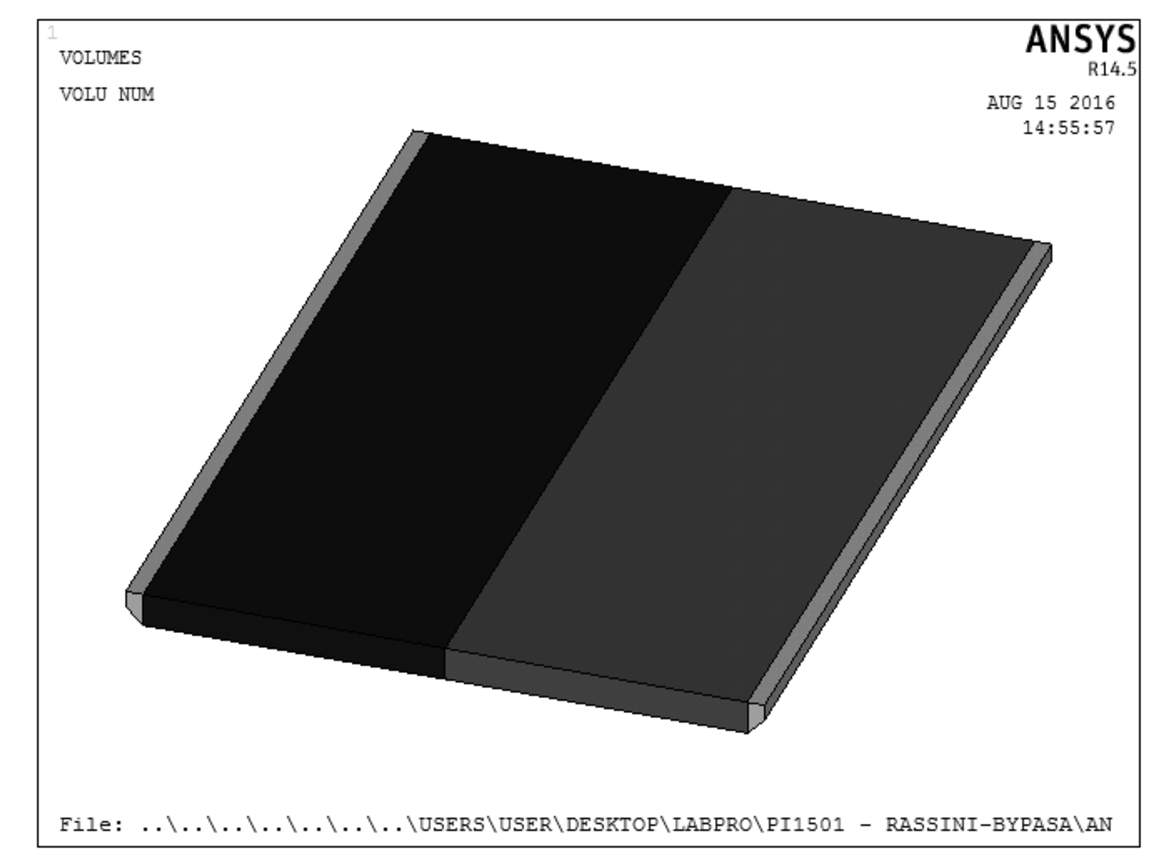
\includegraphics[scale=0.6]{src/ch3/blank_segmentado.png}
\captionof{figure}{Blank segmentado en cuatro regiones}
\label{fig:blank_seg}
\end{center}


% Mallado del ensamble 01

\begin{center}
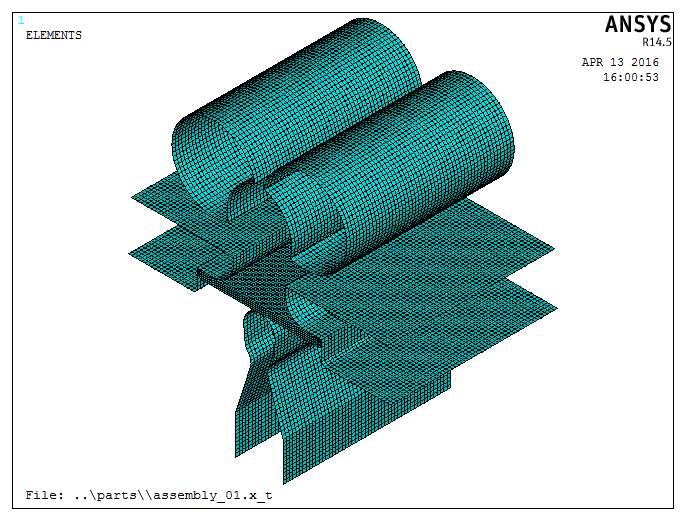
\includegraphics[scale=0.6]{src/ch3/mesh_assembly_01.png}
\captionof{figure}{Mallado del ensamble, primer paso}
\label{fig:mesh_assembly01}
\end{center}

% Mallado del ensamble 01
\begin{center}
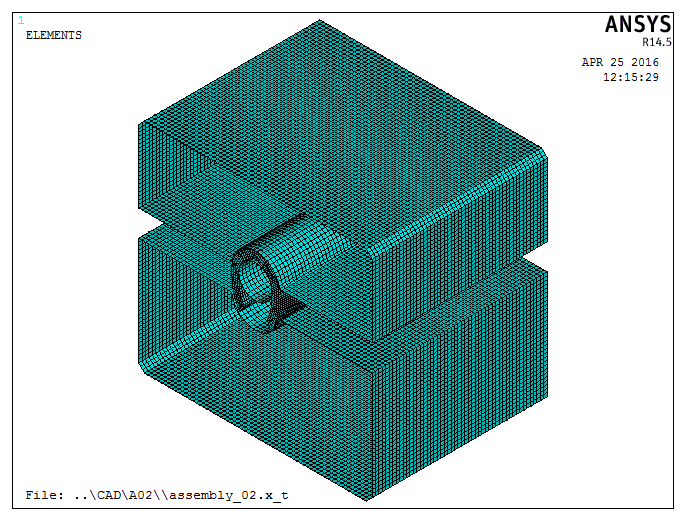
\includegraphics[scale=0.6]{src/ch3/mesh_assembly_02.png}
\captionof{figure}{Mallado del ensamble, segundo paso}
\label{fig:mesh_assembly02}
\end{center}

En las tabla \ref{tab:elements_and_nodes} se muestra el número de nodos y elementos obtenidos 
para cada uno de los ensambles.

\begin{table}[h]
\centering
\caption{Número de nodos y elementos}
\label{}
\begin{tabular}{p{2cm} p{2cm} p{2cm}} \hline
 & Nodos & Elementos \\
\hline
Paso 1 & 52285 & 45348 \\
Paso 2 & 48884 & 42264 \\
\hline
\end{tabular}
\label{tab:elements_and_nodes}
\end{table}


% Condiciones de frontera ==================================================================
\subsection{Condiciones de frontera}

Para efectos de la simulación el blank fue sujetado en el punto medio de cada extremo, 
en las direcciones X y Z, para evitar que se desplace de manera no deseada y con esto 
ayudar en la convergencia de la solución.\\

Para los componentes del troquel, al ser cuerpos rígidos la mayoría de sus
restricciones fueron consideradas en la definición del material. En el caso de los
formadores superiores, sólo se especificaron los desplazamientos en la dirección
vertical Y, se utilizaron arreglos unidimensionales para especificar la relación
tiempo-desplazamiento, en todos los casos se especificó como desplazamiento de
cuerpo rígido en la dirección Y (\texttt{RBUY}), aplicándose esta condición a cada uno de los
componentes.\\

La relación tiempo-desplazamiento se definió utilizando una función de tipo
\textit{smooth-step}, cuya forma general es $f(t) = A(Bt^2 - Ct^3)$ , donde
$A$, $B$ y $C$ son constantes a ajustar para el requerimiento de desplazamiento total,
se caracteriza por tener un crecimiento lento al principio y final del intervalo
especificado, implicando una velocidad reducida de los formadores al principio y final 
del recorrido, con la finalidad de que esto facilite la estabilización y convergencia
del análisis.\\

En la figura \ref{fig:smooth_displacement} se muestra la gráfica del tiempo-desplazamiento 
utilizado en el primer paso del troquel. Para el segundo caso se utilizó una curva 
similar, con algunas variaciones en las constantes para disminuir la amplitud o valor máximo.\\


\begin{apdl}
*DIM,tiempo,ARRAY,400
*DIM,desplazamiento,ARRAY,400

*DO,ii,1,400
	tiempo(ii)=ii/2E3
*ENDDO

_k1 = 3.8E-7
_k2 = 1.15E-4
_k3 = -1.22

*DO,jj,1,200
	desplazamiento(jj)= _k3*(_k2*jj**2 - _k1*jj**3) - (_k3*(_k2 - _k1))
*ENDDO

*DO,kk,1,200
	desplazamiento(200+kk) = (-1)*_k3*(_k2*kk**2 - _k1*kk**3) + (_k3*(_k2*200**2 - _k1*200**3))
*ENDDO

*vplot,tiempo,desplazamiento
\end{apdl}


\begin{center}
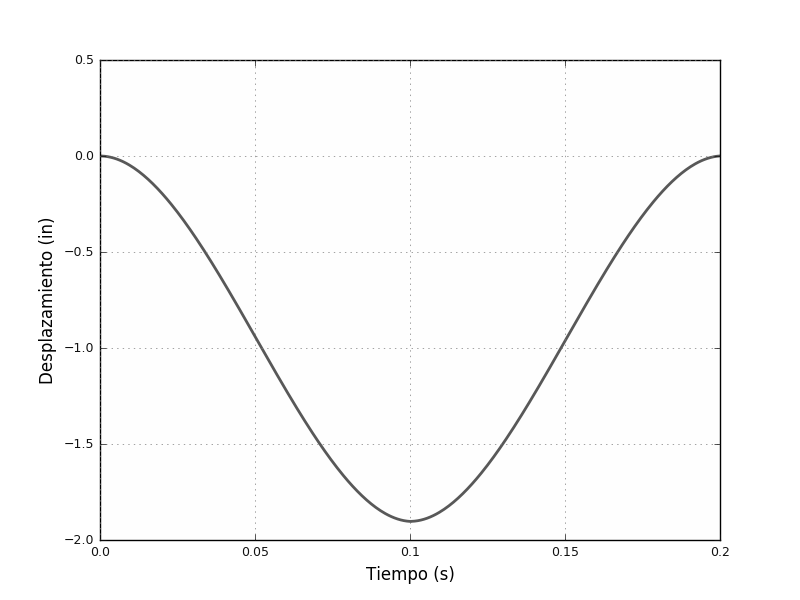
\includegraphics[scale=0.6]{src/ch3/smooth_displacement.png}
\captionof{figure}{Vector de tiempo desplazamiento}
\label{fig:smooth_displacement}
\end{center}



% ==================================== CONTACTOS ============================================
\subsection{Contactos}

En la definición de contactos se utilizó un tipo de contacto superficie a superficie
general. El programa de simulación utiliza los coeficientes de fricción 
estático (FS) y dinámico (FD) para la formulación del coeficiente friccional ($\mu_c$),
que viene dado por la ecuación :

\begin{equation}
\mu_c = FD + (FS - FD) e^{-DCv_{rel}}
\end{equation}

Donde $DC$ es el coeficiente de decaimiento exponencial y $v_{rel}$ la velocidad relativa
entre las superficies en contacto ~\cite{lsdyna-manual}. Los valores del coeficiente de fricción estático
y dinámico se establecieron en 0.2 y 0.1, respectivamente [REVISAR REFERENCIA A HANDBOOK DATA]. 
En la simulación del segundo paso se utilizó el contacto de tipo Single Surface (SS) para tomar en
cuenta el contacto del blank con él mismo (cerrado del tubo) ~\cite{lsdyna-manual}, utilizando
también los parámetros de fricción indicados anteriormente.


\section{Análisis experimental}


